\documentclass[english,ngerman,BCOR=6mm,cdgeometry=no,DIV=13]{tudscrreprt}

\usepackage[T1]{fontenc}
\usepackage[utf8]{inputenc}

\usepackage[ngerman]{babel}
\usepackage[babel,german=quotes]{csquotes}

\usepackage{isodate}
\usepackage{enumerate}
\usepackage{tudcolors}
\usepackage{graphicx}
\usepackage{float}
\usepackage{amsmath}



% Zeilenabstand 1.2-zeilig
\usepackage{setspace}
\setstretch{1.2}

\usepackage{hyperref}
\hypersetup{colorlinks=true, linkcolor=black, citecolor=tudaccent1, menucolor=black,
	urlcolor=tudaccent5} %Verknüpfung nicht umrandet, Verknüpfung von Tabellen/Grafiken/...


%\usepackage[style=apa]{biblatex}
\usepackage[style=apa,backend=biber]{biblatex}
\addbibresource{references.bib}



\begin{document}
\faculty{Fakultät Umweltwissenschaften}
\department{Fachrichtung Hydrowissenschaften}
\institute{Institut für Hydrobiologie}
\chair{Professur für Limnologie (Gewässerökologie)}

\author{Lisa Wasseramsel}
\course{M.Sc. Hydrobiologie}
\title{Entwicklung einer Universalmethode zur Umsetzung der Wassserrahmenrichtlinie}

%\thesis{master} % aktivieren, falls Masterarbeit, bei Bachelor analog
\subject{Berufspraktikumsbericht} % Zeile bei Bachelor- und Masterarbeiten löschen

\graduation[M.Sc.]{Master of Science}
%\dateofbirth{02.01.2001}  % Optional
%\placeofbirth{Dresden}    % Optional

\referee{Prof. Annegret Clearwater (TU Dresden)\and
        Dr. Michael Fischer (Umweltforschungszentrum)}

\supervisor{Dipl.-Biol. Luise Salomon}

\date{24.05.2024}
%\defensedate{10.09.2024}  % Optional


\maketitle
\TUDoption{abstract}{section,multiple}

\begin{abstract}[english,pagestyle=empty.tudheadings]

The English abstract should briefly summarize task, methods and main results.

Lorem ipsum dolor sit amet, consetetur sadipscing elitr, sed diam nonumy eirmod
tempor invidunt ut labore et dolore magna aliquyam erat, sed diam voluptua.
At vero eos et accusam et justo duo dolores et ea rebum.

\nextabstract[ngerman] % ngerman steht fuer neue Rechtschreibung

Lorem ipsum dolor sit amet, consetetur sadipscing elitr, sed diam nonumy eirmod
tempor invidunt ut labore et dolore magna aliquyam erat, sed diam voluptua.
At vero eos et accusam et justo duo dolores et ea rebum.

\end{abstract}


\break
{\hypersetup{linkcolor=black}
\tableofcontents

\break

\addcontentsline{toc}{chapter}{Abbildungsverzeichnis}
\listoffigures

\addcontentsline{toc}{chapter}{Tabellenverzeichnis}
\listoftables

\break
}


\chapter{Einleitung}

Diese Formatvorlage basiert auf der srcreprt-Klasse aus dem TUD-Script-Paket von
Falk Hanisch.

Es fehlen noch Beispiele für Maßeinheiten und chemische Formeln, außerdem soll
noch eine englische Variante erstellt werden.


Lorem ipsum dolor sit amet, consetetur sadipscing elitr, sed diam nonumy eirmod
tempor invidunt ut labore et dolore magna aliquyam erat, sed diam voluptua. At
vero eos et accusam et justo duo dolores et ea rebum. Stet clita kasd gubergren,
no sea takimata sanctus est Lorem ipsum dolor sit amet. Lorem ipsum dolor sit
amet, consetetur sadipscing elitr, sed diam nonumy eirmod tempor invidunt ut
labore et dolore magna aliquyam erat, sed diam voluptua. At vero eos et accusam
et justo duo dolores et ea rebum. Stet clita kasd gubergren, no sea takimata
sanctus est Lorem ipsum dolor sit amet (siehe Abbildung \ref{fig:fig_1}).

\chapter{Methoden}

\section{Untersuchungsgebiet}

\section{Gewässerbewertung}

\section{Statistische Analyse}

Die statistische Analyse wurde mit \textbf{R} \parencite{r-core-2024} und RStudio
\parencite{rstudio-2024} durchgeführt. Für die Grafiken
wurde das Paket \textbf{ggplot2} verwendet \parencite{wickham-ggplot2-2016}.


\chapter{Ergebnisse}

Test von Umlauten und Sonderzeichen äöü ÄÖÜ ßßß µ @ €. Dieser Test soll zeigen,
ob die Schriftarten richtig funktionieren, wenn der Text im UTF-8-Format
abgespeichert wurde.

\begin{figure}
	\centering
	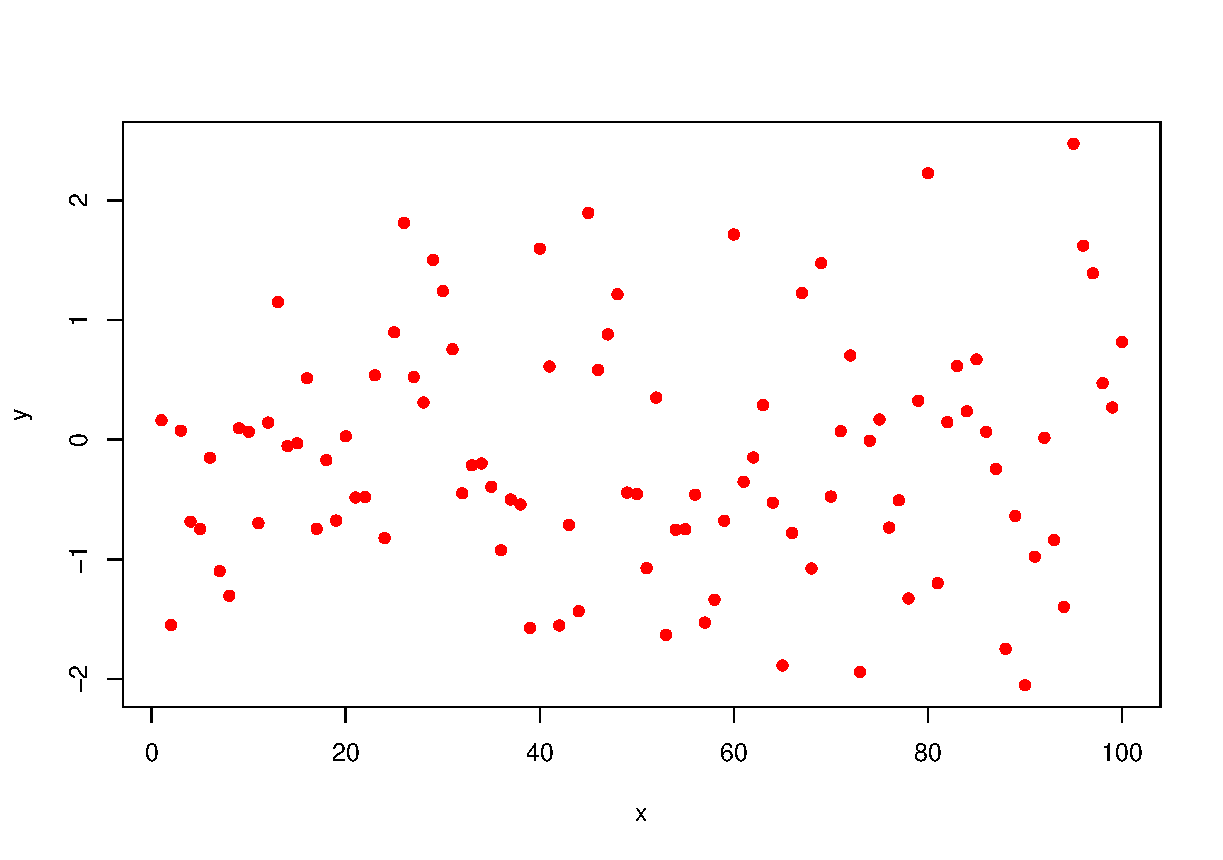
\includegraphics[width=\textwidth]{pdf-plot.pdf}
	\caption[Kurzfassung des Abbildungstitels]{Langfassung des Abbildungstitels,
	         meistens 2-5 Zeilen}\label{fig:fig_1}
\end{figure}

\begin{table}
	\centering
	\caption[Kurzfassung der Tabellenüberschrft]{Langfassung der Tabellenüberschrift,
	        im Regelfall mehrere Zeilen. Es sollten insbesondere Abkürzungen erklärt werden.}
	\label{tab:my_label}
	\begin{tabular}{lll}\hline
		Name & Probenahmestelle & Wert\\\hline
		Temperatur & 1  & 14  \\
		Sauerstof & 2  & 16 \\
		Trübung & 3 & 15 \\ \hline
	\end{tabular}
\end{table}

\chapter{Diskussion}

Hier werden die Aufgaben udn Hypothesen aus der Einleitung aufgegriffen und
argumentativ untersetzt. Potentielle Defizite und Fehler werden eingeräumt und
eingeordnet. Es sollte das Positive herausgerabeitet werden, außer wenn alles
schief gegangen ist.

\chapter{Danksagung}

Die Danksagung kann individuell gestaltet werden. Wichtig ist vor allem,
Praxispartnern zu danken und den Leuten oder Organisationen, von denen man
finanziellen Support oder Daten bekommen hat. Bei BMBF-, DFG-, EU- und anderen
Projekten ist die Nennung des Förderkennzeichens in den Förderrichtlinien
vorgeschrieben.


\printbibliography


\end{document}
